\subsection{Ley de Gustaffson}

\begin{frame}[t]{Planteamiento}
\begin{itemize}
\item La Ley de Amdahl enfatiza el aspecto más negativo del procesamiento paralelo.
\item Sin embargo:
  \begin{itemize}
    \item Las máquinas paralelas se usan para resolver grandes problemas (meteorología, biología molecular, \ldots).
    \item Un computador secuencial nunca podría ejecutar un gran programa paralelo.
    \item No tendría capacidad para ello.
  \end{itemize}
\end{itemize}
\vfill
\[
S = \frac{T_s}{T_p}
\]
\end{frame}

\begin{frame}[t]{Aceleración proporcional}
\begin{itemize}
  \item La cantidad de trabajo que se puede hacer en paralelo varía linealmente con el número de procesadores.
    \begin{itemize}
      \item Con más procesadores se pueden acometer problemas de mayor coste computacional
  \end{itemize}
  \item Un problema con una porción $\alpha$ no paralela (sobre el tiempo total $T$), tardará en una máquina paralela:
\[
T_p = \alpha T + (1-\alpha) T
\]
  \item El mismo problema ejecutado en una máquina secuencial tardaría:
\[
T_s = \alpha T + (1-\alpha) p T
\]
  \item Y por tanto:
\[
S = \frac{T_s}{T_p} = 
\frac{\alpha T + (1-\alpha) p T}{T} = \alpha + (1-\alpha) p =
p + \alpha (1 - p)
\]
\end{itemize}
\end{frame}

\begin{frame}[t]{Efectos de la Ley de Gustaffson}
\begin{itemize}
  \item La ley dede Gustafson asume que la parte secuencial (no paralelizable) disminuye con el tamaño del problema.
    \begin{itemize}
      \item Cuando el problema crece se puede aproximar el paralelismo lineal (S$\approx$p).
    \end{itemize}
  \vfill
  \item El paralelismo permite atacar problemas mayores.
\end{itemize}
\end{frame}

\begin{frame}[t]{Evolución de speedup}
\begin{tikzpicture}
\begin{axis}[xlabel={\tiny procesadores},ylabel=speedup, 
minor y tick num=1,
legend style = {
at={(1.02, 1)},
anchor=north west
},
width=0.85\textwidth, height=0.85\textheight,
xmin=0,xmax=128,
ymin=0,ymax=128]
\addplot [domain=1:128,color=red,very thick] {x + 0.5 * (1-x)};
\addlegendentry{$\alpha$=0.5}
\addplot [domain=1:128,color=orange,very thick] {x + 0.25 * (1-x)};
\addlegendentry{$\alpha$=0.25}
\addplot [domain=1:128,color=green, very thick] {x + 0.2 * (1-x)};
\addlegendentry{$\alpha$=0.2}
\addplot [domain=1:128,color=yellow, very thick] {x + 0.1 * (1-x)};
\addlegendentry{$\alpha$=0.1}
\addplot [domain=1:128, color=blue, very thick] {x};
\addlegendentry{lineal}
\end{axis}
\end{tikzpicture}
\end{frame}

